% ABSA project report - ACL 2023 format, single LaTeX file.
% Compile with pdfLaTeX (e.g. Overleaf: upload this file, acl2023.sty and the figures/ folder).
% Generated by report/make_report.py (the same text is also written to ABSA_Report.docx).
\pdfoutput=1
\documentclass[11pt]{article}
\usepackage[final]{acl2023}
\usepackage{times}
\usepackage{latexsym}
\usepackage[T1]{fontenc}
\usepackage[utf8]{inputenc}
\usepackage{microtype}
\usepackage{inconsolata}
\usepackage{booktabs}
\usepackage{graphicx}
\usepackage{amsmath}

\title{Aspect-Based Sentiment Analysis of Product Reviews: Comparing Traditional and Transformer Models Within and Across Datasets}
\author{Mrigank \\ Roll No. 230150018 \And Varshit \\ Roll No. 230150023 \And Jeshwanth \\ Roll No. 230150011}
\begin{document}
\maketitle
\begin{abstract}
A single product review often praises one part of a product and complains about another. Aspect-based sentiment analysis (ABSA) handles this by finding the aspects a reviewer talks about and working out how the reviewer feels about each one. In this project we built an ABSA pipeline for both steps, aspect term extraction and aspect-level sentiment classification, and used it to compare a TF-IDF baseline with fine-tuned BERT and RoBERTa models on SemEval-2014 Laptops and MAMS. Every model was tested on its own dataset and on the other one. Our first round of fine-tuning already beat TF-IDF by 16.8 macro-F1 points on Laptops and 13.7 on MAMS, but the training curves showed heavy over-fitting and a classifier that had no idea where the aspect was in the sentence. In a second round we addressed this with aspect markers and aspect pooling, label smoothing, adversarial training, layer-wise learning rates and constrained decoding, and we also tried RoBERTa-large. Our best models reach 79.9 macro-F1 on Laptops and 85.1 on MAMS. Transfer between the datasets turned out to be one-sided: models trained on MAMS do reasonably well on Laptops, but not the other way round, and aspect extraction hardly transfers at all. The biggest gain from the second round came on sentences that mix positive and negative opinions, which were the hardest cases for our first models.
\end{abstract}

\section{Introduction}
If you read reviews before buying a laptop, you have probably come across sentences like \textit{``The laptop has an excellent display, but the battery life is disappointing.''} Is that a positive review or a negative one? It is both, and neither. A standard sentiment classifier has to choose one label for the whole sentence, and whichever label it chooses, the useful part of the message is lost. What a buyer, or the company that made the laptop, actually wants to know is that the display is good and the battery is not.

Aspect-based sentiment analysis works at this finer level \citep{hu2004mining,pontiki2014semeval}. It is usually split into two steps. \textbf{Aspect term extraction (ATE)} finds the words that name a part or a property of the product, such as \textit{battery life} or \textit{keyboard}. We treat it as sequence labelling with BIO tags. \textbf{Aspect-level sentiment classification (ASC)} then takes the sentence together with one of its aspects and decides whether the opinion about that aspect is positive, negative or neutral. The same sentence comes back once for every aspect it contains, and the model has to give a different answer depending on which aspect it is asked about.

We set out to answer three questions:

\begin{enumerate}
\setlength\itemsep{0em}
\item How much do pre-trained Transformer models gain over a TF-IDF model with a linear classifier, on both steps?
\item Does a model trained on one ABSA dataset still work on a different one?
\item Which sentences are still hard, and can we fix some of those errors by changing the way we train?
\end{enumerate}

We used two public datasets. SemEval-2014 Task 4 Laptops \citep{pontiki2014semeval} is the standard benchmark for product reviews. MAMS \citep{jiang2019mams} contains restaurant reviews and was built so that every sentence has at least two aspects with different sentiments. We trained each model on one dataset and tested it on both, which gives two in-domain and two cross-dataset settings.

The work happened in two rounds. In the first round (v1) we trained the baselines and a standard Transformer set-up. Looking at the training curves and the errors showed some clear problems, so we ran a second round (v2) in which each change targets one of them. In short, this report covers:

\begin{itemize}
\setlength\itemsep{0em}
\item a reproducible pipeline that puts both datasets into one format, trains and evaluates every model, and also scores the full extract-then-classify system;
\item a fair comparison of TF-IDF with logistic regression and SVM against BERT-base and RoBERTa-base, on the same splits and metrics, in four train/test settings;
\item a second training round based on what the v1 curves showed, run on the same backbone as v1 so that the effect of the new recipe can be separated from the effect of a bigger model;
\item an error analysis that groups test examples by negation, contrast, several aspects, mixed polarities, implicit sentiment and distant opinion words.
\end{itemize}

\section{Related Work}
\textbf{Lexicons and hand-made features.} Early opinion mining relied on lists of sentiment words. \citet{turney2002thumbs} estimated whether a phrase is positive or negative from how often it appears near words such as ``excellent'' and ``poor''. \citet{hu2004mining} mined frequent noun phrases from customer reviews as product features and gave each one the polarity of the opinion words around it. The surveys by \citet{pang2008opinion}, \citet{liu2012sentiment}, \citet{liu2015sentiment} and \citet{medhat2014sentiment} describe how these ideas grew into supervised classifiers over bag-of-words features. Such models are fast and easy to understand, but they cannot tell which opinion word belongs to which aspect, and that is exactly what ABSA needs.

\textbf{Benchmarks.} The SemEval-2014 shared task \citep{pontiki2014semeval} released laptop and restaurant reviews annotated with aspect terms, their positions and their polarity, and SemEval-2016 \citep{pontiki2016semeval} added more languages and domains. \citet{jiang2019mams} noticed that most SemEval sentences have only one aspect, or several aspects with the same polarity, so a model can score well just by reading the overall tone of the sentence. Their MAMS dataset removes that shortcut: every sentence has several aspects, and they disagree.

\textbf{Transformers.} The Transformer \citep{vaswani2017attention} and pre-trained encoders such as BERT \citep{devlin2019bert} and RoBERTa \citep{liu2019roberta} changed most of NLP, and ABSA was no exception. \citet{sun2019utilizing} turned aspect sentiment into a sentence-pair task by giving BERT the sentence together with a short auxiliary sentence about the aspect, and our input format follows the same idea. \citet{rietzler2020adapt} showed that further pre-training on in-domain reviews helps, and they also looked at transfer between laptops and restaurants. Sentence-BERT \citep{reimers2019sentence} trains BERT to produce embeddings for comparing sentences. We did not use it, because in our task the aspect and the sentence need to be read together by a single encoder.

\textbf{Training techniques.} Marking a target span in the input text is a simple way to tell an encoder what a prediction is about. \citet{zhou2022improved} found that plain punctuation marks work well for this in relation extraction, and we borrowed that idea. Adversarial training on word embeddings \citep{miyato2017adversarial} and label smoothing \citep{szegedy2016rethinking} are general ways of reducing over-fitting. None of these techniques is new. What we wanted to find out was which of them actually help in our setting.

\section{Data}
\textbf{SemEval-2014 Laptops.} The training file has 3,045 sentences and the test file 800. Each aspect term comes with its character positions and one of four labels: positive, negative, neutral or conflict. We kept sentences without any aspect for extraction, because the tagger also has to learn when there is nothing to extract. The conflict label is rare (45 training cases) and does not exist in MAMS, so we removed those cases from the sentiment task. That way every experiment uses the same three classes, which the cross-dataset tests need. SemEval has no validation set, so we held out a random 10\% of the training \textit{sentences} (304 of them). Splitting by sentence rather than by aspect makes sure that no sentence ends up in both training and validation.

\textbf{MAMS.} We used the aspect-term version of MAMS from the authors' GitHub repository. It comes with its own training, validation and test splits of 4,297, 500 and 500 sentences, all taken from restaurant reviews.

\begin{table}[t]
\centering
\small
\begin{tabular}{lcccccc}
\toprule
Corpus & Split & Sentences & Aspects & Pos & Neg & Neu \\
\midrule
Laptops & train & 2,741 & 2,092 & 889 & 786 & 417 \\
Laptops & val & 304 & 221 & 98 & 80 & 43 \\
Laptops & test & 800 & 638 & 341 & 128 & 169 \\
\midrule
MAMS & train & 4,297 & 11,186 & 3,380 & 2,764 & 5,042 \\
MAMS & val & 500 & 1,332 & 403 & 325 & 604 \\
MAMS & test & 500 & 1,336 & 400 & 329 & 607 \\
\bottomrule
\end{tabular}
\caption{Size of the two datasets after preprocessing. ``Aspects'' counts sentence--aspect pairs labelled positive, negative or neutral (the SemEval conflict label is removed). The Laptops validation split is a random 10\% of the original training sentences.}
\label{tab:datasets}
\end{table}

\textbf{Preprocessing.} Both datasets are XML files with the same basic structure, so one parser handles both. We split each sentence into word tokens with a regular expression that keeps track of character positions, and then mapped each aspect's character span onto the tokens it covers to get the BIO tags. The same records also give one sentence--aspect pair per labelled aspect for the sentiment task. Parsing and tagging run in parallel on all CPU cores and the result is cached, so this step takes a few seconds the first time and no time at all after that.

\begin{figure}[t]
\centering
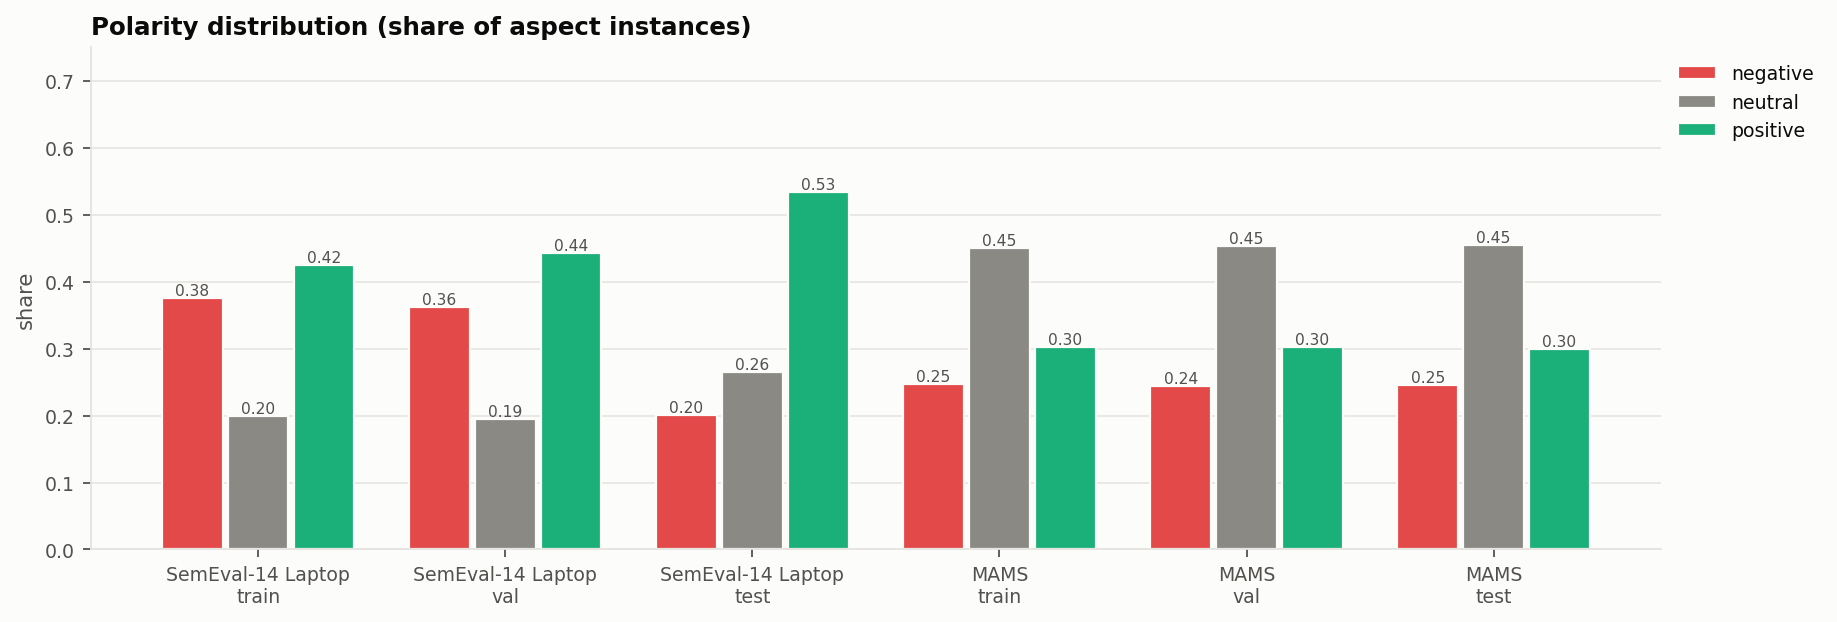
\includegraphics[width=1\columnwidth]{figures/polarity_distribution.png}
\caption{Share of positive, negative and neutral aspects in each dataset and split.}
\label{fig:polarity}
\end{figure}

\textbf{What the data looks like.} Table~\ref{tab:datasets} gives the sizes, and Figure~\ref{fig:polarity} and Figure~\ref{fig:eda} show how the two datasets differ. They differ in almost every way that matters for this task:

\begin{itemize}
\setlength\itemsep{0em}
\item \textbf{Aspects per sentence.} Only 19\% of Laptops sentences have more than one aspect, and only 11\% of the sentences with aspects mix polarities. In MAMS both numbers are 100\%. A MAMS sentence has 2.6 aspects on average, compared with 1.6 for Laptops.
\item \textbf{Labels.} Laptops is mostly positive (42\% of training aspects, with only 20\% neutral). MAMS leans the other way: 45\% of its aspects are neutral.
\item \textbf{Length.} MAMS sentences are longer, 26.9 words on average against 16.8.
\item \textbf{Vocabulary.} The two training sets contain 879 and 2410 different aspect terms, and only 26 of them appear in both (a Jaccard overlap of 0.008). Laptop reviews talk about the \textit{battery}, \textit{screen} and \textit{keyboard}, restaurant reviews about the \textit{food}, \textit{staff} and \textit{service}.
\end{itemize}

Even before training anything, these numbers suggested that sentiment would transfer unevenly between the two datasets and that extraction would hardly transfer at all.

\begin{figure*}[t]
\centering
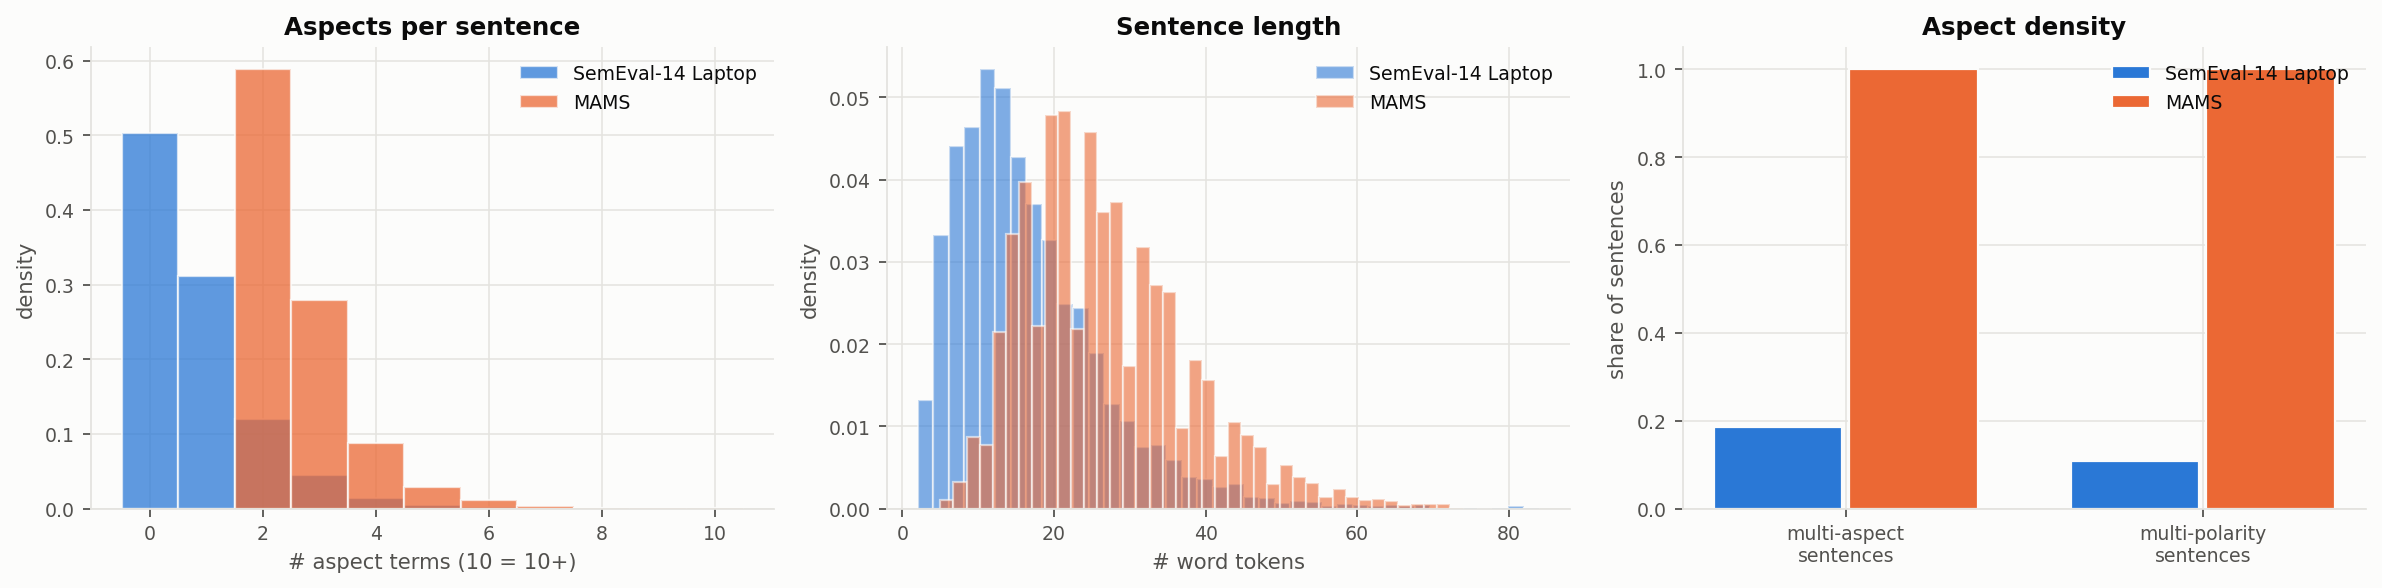
\includegraphics[width=1\textwidth]{figures/aspects_and_lengths.png}
\caption{Aspects per sentence, sentence length, and how many sentences have several aspects or several polarities.}
\label{fig:eda}
\end{figure*}

\section{Methods}
\subsection{Task set-up}
For extraction, each word gets one of three tags: B starts an aspect term, I continues it, and O marks everything else. We turn the predicted tags back into spans and count a span as correct only if it matches a gold span exactly. For sentiment, the input is a sentence plus one aspect from it, and the output is positive, negative or neutral.

\subsection{Traditional baselines}
\textbf{Sentiment.} A bag-of-words model sees the whole sentence but has no way of knowing which aspect we are asking about. To give it a fair chance, we built three groups of TF-IDF features and joined them: unigrams and bigrams of the full sentence; unigrams and bigrams of a window of six words on either side of the aspect, with each word marked by the side it comes from (so ``not'' before the aspect and ``not'' after it are different features); and the words of the aspect itself. On top of these features we trained logistic regression (LR) and a linear SVM, both with class weights to balance the labels. We picked the regularisation constant C from eight values between 0.01 and 30 using validation macro-F1.

\textbf{Extraction.} The traditional tagger is a logistic regression classifier that labels one word at a time. Its features are the lower-cased word, its prefixes and suffixes, a word-shape pattern, capitalisation and digit flags, the position of the word, the two words on each side, and word bigrams. To keep the names short we list it as TF-IDF+LR in the extraction tables, even though its features are simple indicators rather than TF-IDF weights.

\subsection{Transformer models (v1)}
We fine-tuned BERT-base-uncased \citep{devlin2019bert} and RoBERTa-base \citep{liu2019roberta}. For sentiment, the input is the sentence and the aspect as a pair, ``[CLS] sentence [SEP] aspect [SEP]'', as in \citet{sun2019utilizing}, and a linear layer on the final [CLS] vector predicts the label. For extraction, a linear layer on every token predicts a BIO tag. When a word is split into several sub-word pieces, only the first piece is labelled and the rest are left out of the loss. Both tasks use cross-entropy loss and the AdamW optimiser with weight decay 0.01, a learning rate that warms up over the first 10\% of the steps and then decays linearly, and gradient clipping at 1.0.

\subsection{Improved recipe (v2)}
The v1 results, described in the next sections, showed four problems. The models over-fitted badly, the sentiment classifier was never told where the aspect was, the neutral class was weak, and choosing the best checkpoint on the small Laptops validation set was noisy. The second round makes the following changes.

\textbf{Aspect markers and aspect pooling.} We wrap the aspect inside the sentence with plain \# characters, for example ``the \# battery life \# is disappointing'', following the idea of \citet{zhou2022improved}. The aspect is still passed as the second segment as well. Instead of using only the [CLS] vector, the classifier now reads

\begin{equation}
\mathbf{z} = \big[\,\mathbf{h}_{\texttt{CLS}} \,;\, \tfrac{1}{|A|}\textstyle\sum_{t \in A} \mathbf{h}_t\,\big]
\end{equation}
where A holds the positions of the aspect's sub-word pieces inside the sentence, which we find from the tokenizer's character offsets. The vector z goes through a small two-layer head with dropout. Put simply, the head is now told which part of the sentence it has to judge, and that matters most when a sentence contains several aspects.

\textbf{Label smoothing.} Instead of a hard target of 1 for the correct class, we use 0.9 and share the remaining 0.1 between the other two classes \citep{szegedy2016rethinking}. This keeps the model from becoming over-confident on the training examples.

\textbf{Adversarial training.} We use the fast gradient method \citep{miyato2017adversarial}. After the normal backward pass we push the word-embedding matrix a small step ($\epsilon$ = 0.5) in the direction that increases the loss, run a second forward and backward pass on the shifted embeddings, add up the gradients, and then put the embeddings back. The model learns to give the same answer when its input is slightly disturbed.

\textbf{Layer-wise learning rates.} Each layer of the encoder trains with a slightly smaller learning rate than the layer above it (a factor of 0.9 per layer for the 12-layer base model and 0.95 for the 24-layer large model). The lower layers, which hold general knowledge about language, therefore change less than the top layers, while the new classification head gets a higher rate.

\textbf{Constrained decoding for extraction.} Instead of picking the best tag for each word on its own, we run the Viterbi algorithm over the word-level probabilities and forbid the transitions O$\to$I and start$\to$I. The output is always a valid BIO sequence.

\textbf{Checkpoint selection and model size.} We now check the validation set four times per epoch instead of twice, use batches of 16 instead of 32, and stop after two epochs without improvement (three for extraction). Finally, we trained RoBERTa-large with the same recipe. It only fits on our 8 GB GPU with gradient checkpointing.

\begin{table}[t]
\centering
\footnotesize
\begin{tabular}{lccccccc}
\toprule
Model & Task & Ep. & BS & LR & LLRD & LS & FGM \\
\midrule
BERT-b v1 & ASC & 6 & 32 & 2e-5 & 1 & 0 & 0 \\
RoBERTa-b v1 & ASC & 6 & 32 & 2e-5 & 1 & 0 & 0 \\
BERT-b v1 & ATE & 8 & 32 & 5e-5 & 1 & 0 & 0 \\
RoBERTa-b v1 & ATE & 8 & 32 & 5e-5 & 1 & 0 & 0 \\
RoBERTa-L v2 & ASC & 4 & 16 & 1.5e-5 & 0.95 & 0.1 & 0.5 \\
RoBERTa-b v2 & ASC & 5 & 16 & 3e-5 & 0.9 & 0.1 & 0.5 \\
RoBERTa-L v2 & ATE & 6 & 16 & 2e-5 & 0.95 & 0 & 0.5 \\
RoBERTa-b v2 & ATE & 8 & 16 & 5e-5 & 0.9 & 0 & 0.5 \\
\bottomrule
\end{tabular}
\caption{Fine-tuning settings (b = base, L = large). Ep. is the maximum number of epochs (early stopping usually ends training sooner), BS the batch size, LLRD the layer-wise learning-rate decay, LS label smoothing and FGM the size $\epsilon$ of the adversarial nudge.}
\label{tab:hparams}
\end{table}

\subsection{Implementation}
Everything is written in Python with PyTorch, Hugging Face Transformers, scikit-learn and pandas, and all neural models were trained on one laptop GPU, an NVIDIA RTX 4060 with 8 GB of memory. To keep the GPU busy we load the whole tokenised dataset into GPU memory, cut each batch to the length of its longest sentence, and train in bfloat16 mixed precision. The eight v1 fine-tuning runs took about 15 minutes of training in total and the eight v2 runs about 58 minutes, 20 of which went to RoBERTa-large on MAMS sentiment. The scripts can be resumed if they stop, and a Jupyter notebook reproduces every table and figure in this report.

\section{Experimental Setup}
\textbf{Settings.} Each model is trained on one dataset, tuned on that dataset's validation split, and then tested on the test sets of both datasets. We write the four settings as L$\to$L and M$\to$M (in-domain) and L$\to$M and M$\to$L (cross-dataset), where L stands for Laptops and M for MAMS. The test sets were used only once, after training had finished.

\textbf{Metrics.} For sentiment we report accuracy, macro-averaged precision, recall and F1, the F1 of each class, and confusion matrices. Macro-F1 is our main number, because with uneven labels accuracy can look fine while a small class is handled badly. For extraction we report exact-match span precision, recall and F1. For the full pipeline we pass the aspects found by a tagger to the sentiment model of the same family and compute F1 over (aspect, polarity) pairs, where a pair only counts if both parts are right.

\textbf{Training and model selection.} During training we measured the loss and the main metric on the training and validation sets several times per epoch, and kept the checkpoint with the best validation score (macro-F1 for sentiment, span F1 for extraction). That is the checkpoint we tested. Table~\ref{tab:hparams} lists the settings. Every run uses the same random seed, 42.

\section{Results}
\begin{table*}[t]
\centering
\footnotesize
\begin{tabular}{lcccccccc}
\toprule
 & \multicolumn{4}{c}{Macro-F1} & \multicolumn{4}{c}{Accuracy} \\
\cmidrule(lr){2-5} \cmidrule(lr){6-9}
Model & L$\to$L & M$\to$M & L$\to$M & M$\to$L & L$\to$L & M$\to$M & L$\to$M & M$\to$L \\
\midrule
TF-IDF+LR & 60.7 & 70.3 & 44.6 & 52.3 & 67.1 & 71.5 & 44.8 & 59.2 \\
TF-IDF+SVM & 59.2 & 71.3 & 41.9 & 51.1 & 66.5 & 72.5 & 42.7 & 57.8 \\
BERT-base v1 & 73.2 & 83.3 & 51.8 & 67.7 & 77.6 & 83.7 & 51.6 & 69.9 \\
RoBERTa-base v1 & 77.5 & 84.0 & 48.2 & 72.1 & 80.4 & 84.5 & 48.7 & 75.4 \\
\midrule
RoBERTa-base v2 & 77.9 & 84.5 & \textbf{57.4} & 69.1 & 82.0 & 85.0 & \textbf{58.3} & 72.7 \\
RoBERTa-large v2 & \textbf{79.9} & \textbf{85.1} & 54.2 & \textbf{73.2} & \textbf{83.2} & \textbf{85.6} & 55.6 & \textbf{76.2} \\
\bottomrule
\end{tabular}
\caption{Aspect sentiment results on the test sets (\%). L = Laptops, M = MAMS, and ``L$\to$M'' means trained on Laptops and tested on MAMS. Rows below the line use the v2 recipe. The best value in each column is in bold.}
\label{tab:asc}
\end{table*}

\subsection{Aspect sentiment within a dataset}
Table~\ref{tab:asc} has the main results. In the first round, both Transformers beat both TF-IDF models in every setting. On Laptops, RoBERTa-base reaches 77.5 macro-F1 against 60.7 for TF-IDF+LR, a difference of 16.8 points. On MAMS the difference is 13.7 points (84.0 against 70.3). RoBERTa is clearly better than BERT on Laptops (77.5 against 73.2) and slightly better on MAMS (84.0 against 83.3). The two TF-IDF classifiers are almost tied.

The second round pushed the in-domain numbers further. With the same backbone, RoBERTa-base v2 gets 77.9 on Laptops and 84.5 on MAMS, only 0.4 and 0.5 points above v1. RoBERTa-large v2 does more: 79.9 on Laptops (2.4 points above v1, with 83.2\% accuracy) and 85.1 on MAMS (1.0 points above v1). These are our best in-domain results.

\begin{table}[t]
\centering
\footnotesize
\begin{tabular}{lcccccc}
\toprule
 & \multicolumn{3}{c}{Laptops} & \multicolumn{3}{c}{MAMS} \\
\cmidrule(lr){2-4} \cmidrule(lr){5-7}
Model & Pos & Neg & Neu & Pos & Neg & Neu \\
\midrule
TF-IDF+LR & 80.5 & 53.3 & 48.3 & 64.5 & 69.1 & 77.3 \\
TF-IDF+SVM & 80.2 & 54.9 & 42.5 & 66.4 & 69.3 & 78.0 \\
BERT-base v1 & 87.8 & 71.5 & 60.3 & 83.0 & 81.3 & 85.5 \\
RoBERTa-base v1 & 88.9 & 75.4 & 68.1 & 83.7 & 81.9 & 86.5 \\
RoBERTa-base v2 & 90.7 & \textbf{80.3} & 62.7 & 83.9 & \textbf{82.4} & 87.2 \\
RoBERTa-large v2 & \textbf{91.6} & 78.9 & \textbf{69.1} & \textbf{85.5} & 82.1 & \textbf{87.7} \\
\bottomrule
\end{tabular}
\caption{F1 for each class (\%), in-domain.}
\label{tab:perclass}
\end{table}

Table~\ref{tab:perclass} breaks the scores down by class. On Laptops, neutral is the weakest class for every model: RoBERTa-base v1 reaches 68.1 neutral F1 and RoBERTa-large v2 69.1, while positive F1 is around 90. Neutral aspects are often mentioned in passing, without any opinion words, and the line between a mildly positive remark and a neutral one is blurry even for people. On MAMS, where neutral is the most common label, it is actually the easiest class.

\subsection{Aspect sentiment across datasets}
The cross-dataset columns of Table~\ref{tab:asc}, also drawn as heat maps in Figure~\ref{fig:cross}, show that transfer only works well in one direction. A RoBERTa-base model trained on MAMS scores 72.1 on Laptops, not far from the 77.5 of a model trained on Laptops itself. The same model trained on Laptops scores only 48.2 on MAMS, far below the 84.0 of the in-domain MAMS model. Every model shows the same pattern, TF-IDF included, which tells us that the cause lies in the data rather than in the architecture.

\begin{figure*}[t]
\centering
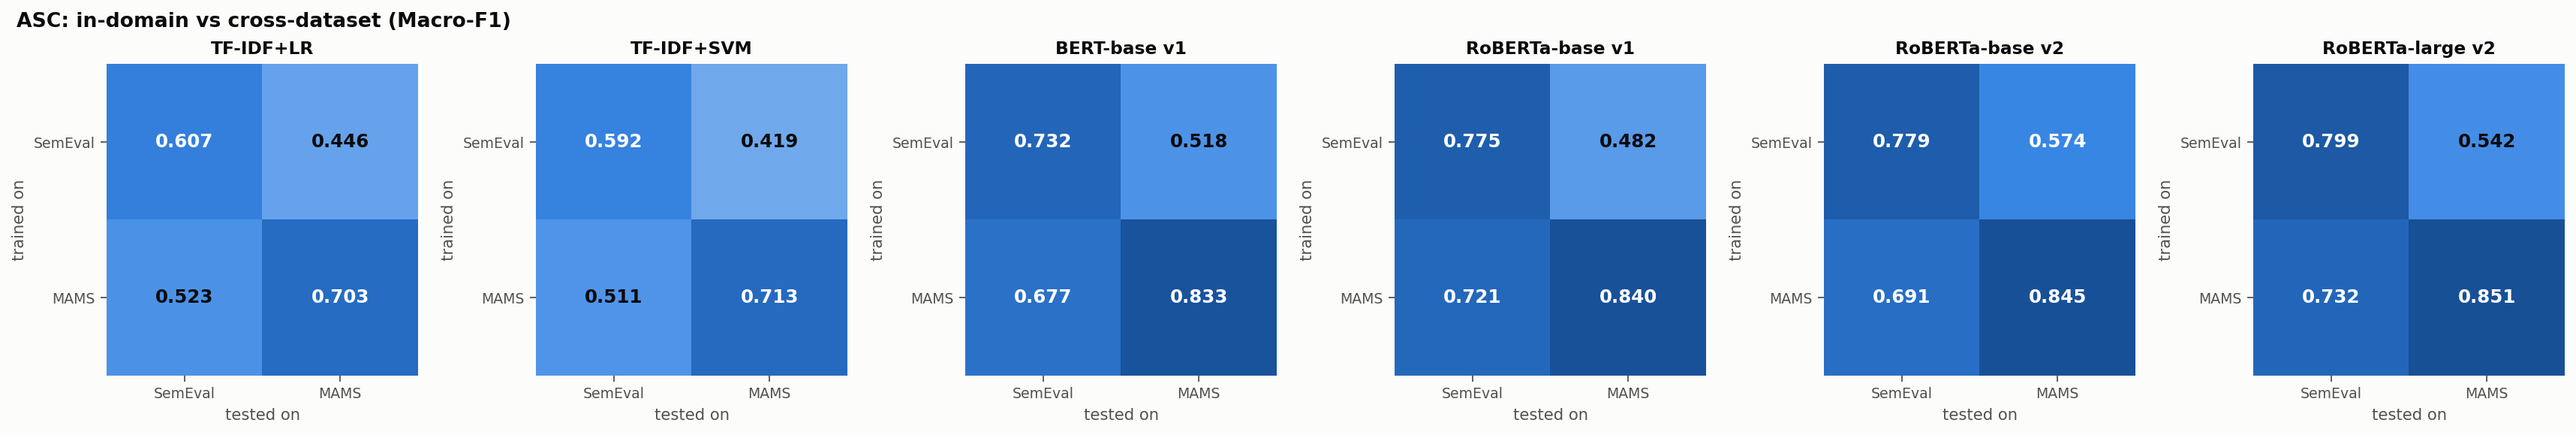
\includegraphics[width=1\textwidth]{figures/asc_cross_dataset_macro_f1.png}
\caption{Sentiment macro-F1 of every model in the four settings. Rows are the training dataset, columns the test dataset.}
\label{fig:cross}
\end{figure*}

We see two reasons. First, about nine out of ten Laptops sentences with aspects express only one sentiment, so a model trained on them can do well by reading the general tone of the sentence. On MAMS, where the aspects of a sentence always disagree, that shortcut breaks. A model trained on MAMS has had to learn to keep aspects apart, and that skill still works on the easier Laptops sentences. Second, the label mix is different. The Laptops model rarely predicts neutral, and in v1 its neutral F1 on MAMS is only 33.1, even though neutral is the most common label there.

The second round helps a lot in the hard direction. RoBERTa-base v2 reaches 57.4 on L$\to$M, 9.2 points above v1, and its neutral F1 on MAMS rises to 40.8. In the other direction the picture is mixed: RoBERTa-base v2 loses 3.0 points on M$\to$L, while RoBERTa-large v2 gains 1.1. Our best cross-dataset results are 57.4 for L$\to$M (RoBERTa-base v2) and 73.2 for M$\to$L (RoBERTa-large v2).

\begin{table*}[t]
\centering
\footnotesize
\begin{tabular}{lcccccccc}
\toprule
 & \multicolumn{3}{c}{Laptops (in-domain)} & \multicolumn{3}{c}{MAMS (in-domain)} & \multicolumn{2}{c}{Cross-dataset F1} \\
\cmidrule(lr){2-4} \cmidrule(lr){5-7} \cmidrule(lr){8-9}
Model & P & R & F1 & P & R & F1 & L$\to$M & M$\to$L \\
\midrule
TF-IDF+LR & 62.5 & 53.8 & 57.8 & 66.8 & 70.6 & 68.6 & 19.6 & 11.1 \\
BERT-base v1 & 80.5 & 82.3 & 81.4 & 71.8 & 78.6 & 75.0 & 24.2 & 31.6 \\
RoBERTa-base v1 & 86.5 & \textbf{85.3} & 85.9 & \textbf{74.2} & 78.4 & 76.2 & \textbf{44.0} & 39.5 \\
\midrule
RoBERTa-base v2 & 85.8 & 83.3 & 84.6 & 73.0 & \textbf{83.8} & \textbf{78.0} & 38.3 & \textbf{41.5} \\
RoBERTa-large v2 & \textbf{88.1} & 84.1 & \textbf{86.1} & 73.4 & 80.5 & 76.8 & 38.1 & 40.3 \\
\bottomrule
\end{tabular}
\caption{Aspect term extraction with exact span matching (\%). The traditional tagger is listed as TF-IDF+LR for short.}
\label{tab:ate}
\end{table*}

\subsection{Aspect term extraction}
Table~\ref{tab:ate} shows the extraction results. Within a domain, the fine-tuned taggers are far ahead of the feature-based one on Laptops (RoBERTa-base v1 reaches 85.9 span F1, against 57.8) and well ahead on MAMS (76.2 against 68.6). The v2 changes made little difference here. Compared with RoBERTa-base v1, the base v2 tagger is 1.4 points lower on Laptops and 1.8 points higher on MAMS, and the large tagger is within one point of v1 on both. Extraction was already strong in v1, so there was not much room left.

Across domains, extraction mostly fails. Trained on Laptops and tested on MAMS, RoBERTa-base v1 reaches 76\% precision but only 31\% recall. The aspects it finds are usually right, but most restaurant aspects (dishes, staff, decor) never appear in laptop reviews, so it simply does not recognise them. The other way round, precision drops to 33\% at 48\% recall, because the MAMS tagger has learned to tag many nouns and over-tags laptop text. With an aspect vocabulary overlap of only 0.008 this is what we expected. Getting extraction to work in a new domain needs at least some text from that domain \citep{rietzler2020adapt}.

\subsection{The full pipeline}
\begin{table}[t]
\centering
\footnotesize
\begin{tabular}{lcccc}
\toprule
Model & L$\to$L & M$\to$M & L$\to$M & M$\to$L \\
\midrule
TF-IDF+LR & 41.4 & 52.1 & 10.8 & 6.5 \\
TF-IDF+SVM & 40.5 & 52.9 & 10.1 & 6.5 \\
BERT-base v1 & 63.5 & 64.2 & 14.2 & 24.6 \\
RoBERTa-base v1 & 69.1 & 65.5 & 27.6 & 29.9 \\
RoBERTa-base v2 & 70.2 & \textbf{67.1} & 28.8 & 30.8 \\
RoBERTa-large v2 & \textbf{70.9} & 66.2 & \textbf{29.5} & \textbf{32.6} \\
\bottomrule
\end{tabular}
\caption{Full pipeline (extract, then classify): F1 over (aspect, polarity) pairs (\%). A pair counts only if both the span and its polarity are right.}
\label{tab:e2e}
\end{table}

Table~\ref{tab:e2e} chains the two steps together. The pair F1 is always lower than either step on its own, since an aspect that the tagger misses can never get the right sentiment. Within a domain, RoBERTa-large v2 reaches 70.9 on Laptops and 66.2 on MAMS, 1.8 and 0.7 points above RoBERTa-base v1, while the TF-IDF pipeline gets 41.4 and 52.1. Across datasets every pipeline stays below 33, held back by extraction. Both v2 models improve the pair F1 in all four settings.

\subsection{How the models learned}
Figure~\ref{fig:curves} shows how RoBERTa learned MAMS sentiment in each round. In v1, training macro-F1 keeps climbing to 98, while validation macro-F1 stops improving early and peaks at 83.1. The validation loss is lowest (0.50) around epoch 1.5 and then climbs back to 0.67. In other words, the model keeps getting more confident about examples it has already seen without getting any better on new ones. On the Laptops validation set, which has only 221 aspects, the score jumped by up to 5.9 points between two checks, so which checkpoint we ended up with was partly luck. These two observations are what led to the changes in v2.

\begin{figure*}[t]
\centering
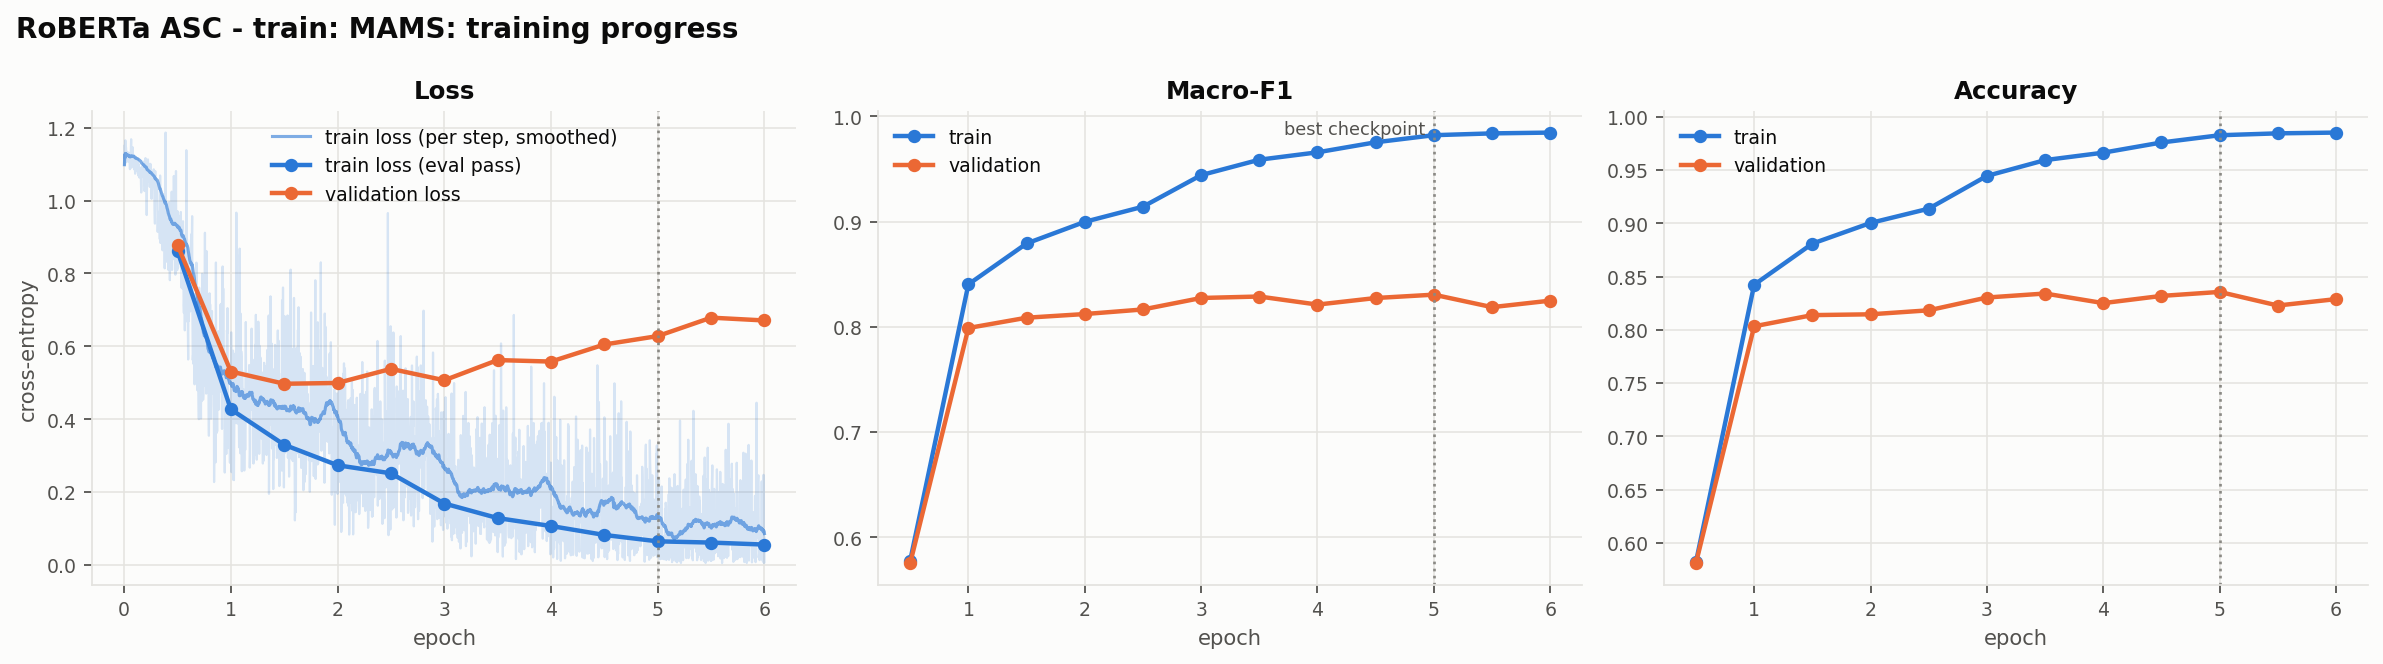
\includegraphics[width=1\textwidth]{figures/v1_curves_roberta_asc_mams.png}
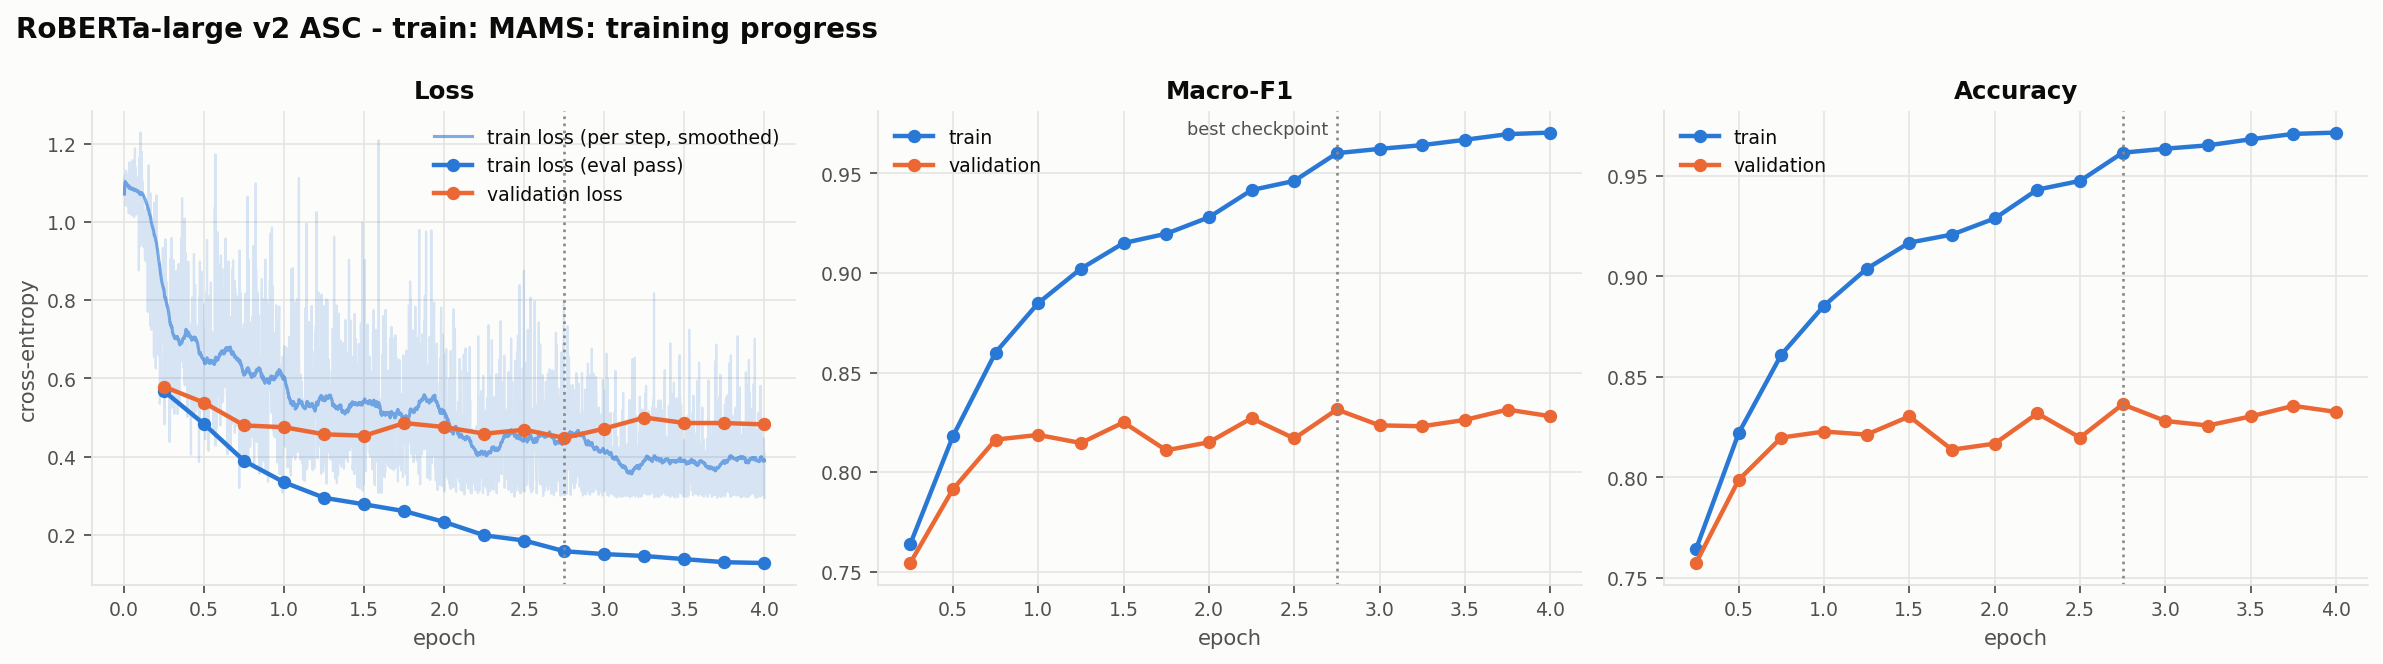
\includegraphics[width=1\textwidth]{figures/v2_curves_large_asc_mams.png}
\caption{Training progress for sentiment on MAMS: RoBERTa-base v1 (top) and RoBERTa-large v2 (bottom). Blue is the training set, orange the validation set, and the dotted line marks the checkpoint that was kept. The faint line is the per-step training loss, which in v2 includes label smoothing.}
\label{fig:curves}
\end{figure*}

\section{From v1 to v2}
\begin{table}[t]
\centering
\footnotesize
\begin{tabular}{lcccc}
\toprule
v2 model & L$\to$L & M$\to$M & L$\to$M & M$\to$L \\
\midrule
\multicolumn{5}{l}{\textit{Sentiment macro-F1}} \\
RoBERTa-base & +0.4 & +0.5 & +9.2 & -3.0 \\
RoBERTa-large & +2.4 & +1.0 & +5.9 & +1.1 \\
\multicolumn{5}{l}{\textit{Sentiment accuracy}} \\
RoBERTa-base & +1.6 & +0.5 & +9.6 & -2.7 \\
RoBERTa-large & +2.8 & +1.1 & +6.9 & +0.8 \\
\multicolumn{5}{l}{\textit{Extraction span F1}} \\
RoBERTa-base & -1.4 & +1.8 & -5.7 & +2.0 \\
RoBERTa-large & +0.2 & +0.6 & -5.9 & +0.8 \\
\multicolumn{5}{l}{\textit{Full pipeline F1}} \\
RoBERTa-base & +1.0 & +1.6 & +1.3 & +0.9 \\
RoBERTa-large & +1.8 & +0.7 & +1.9 & +2.7 \\
\bottomrule
\end{tabular}
\caption{Change in points of each v2 model compared with RoBERTa-base v1, our best v1 model. Positive numbers mean v2 is better.}
\label{tab:delta}
\end{table}

Table~\ref{tab:delta} compares each v2 model with RoBERTa-base v1, our best first-round model, and Figure~\ref{fig:v1v2} puts their validation curves side by side. RoBERTa-base v2 uses the same encoder as v1, so its row shows what the new recipe does on its own. The RoBERTa-large row adds a bigger model on top of that.

\textbf{What worked.} For sentiment, the recipe alone gives only small in-domain gains (0.4 points on Laptops and 0.5 on MAMS) but a large one in the hard L$\to$M setting (9.2 points). The larger encoder adds more in-domain (2.4 points on Laptops and 1.0 on MAMS over v1). RoBERTa-large v2 beats the best v1 model in all four sentiment settings, and both v2 models improve the full-pipeline F1 everywhere. The aspect-pooled head was designed for sentences with several aspects, so it makes sense that its biggest effect shows up in L$\to$M, where every test sentence mixes polarities.

\begin{figure*}[t]
\centering
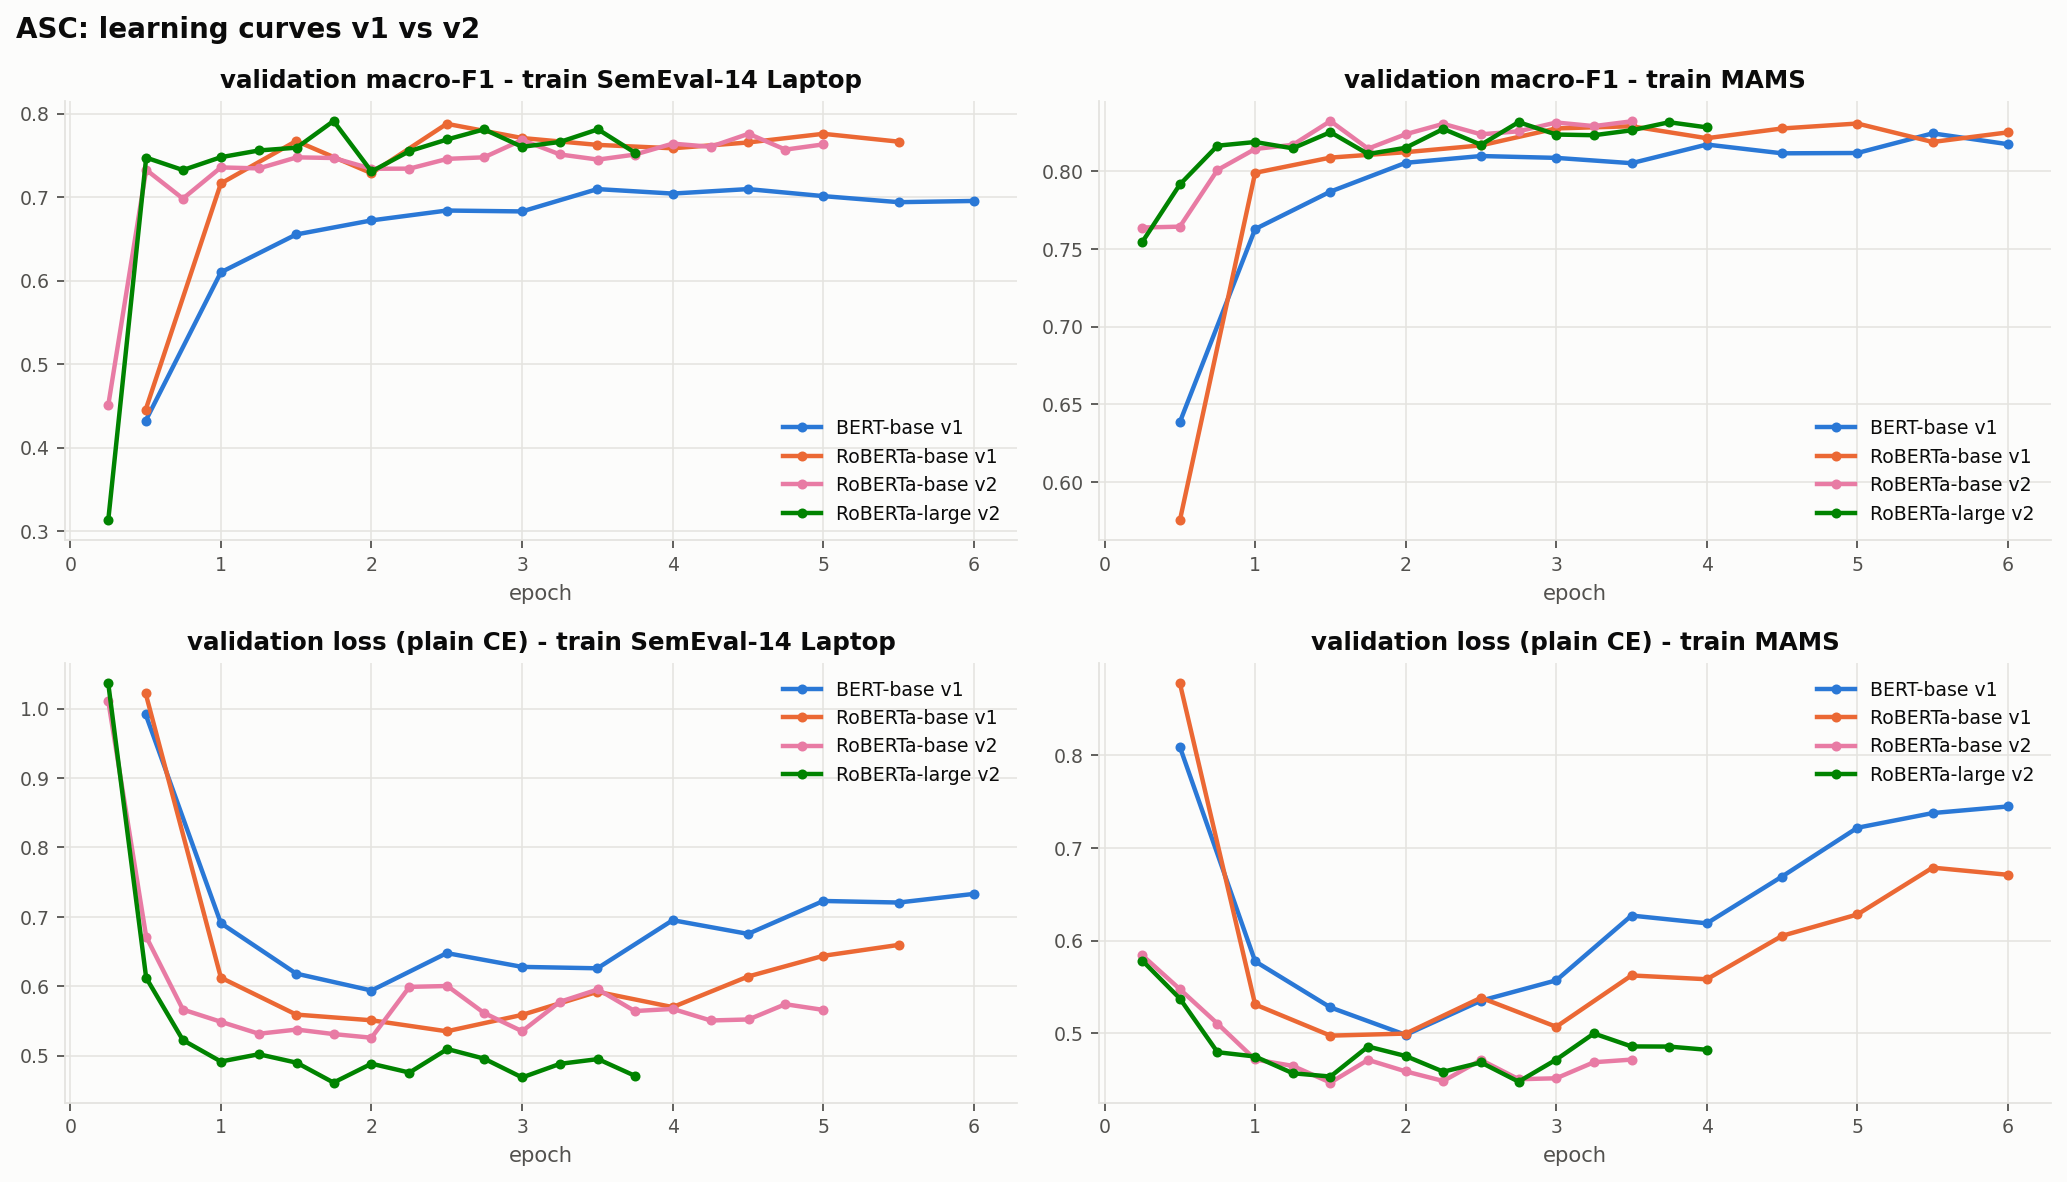
\includegraphics[width=0.8\textwidth]{figures/asc_val_curves_v1_vs_v2.png}
\caption{Validation macro-F1 (top) and validation loss (bottom) while training the sentiment models of both rounds, on Laptops (left) and MAMS (right).}
\label{fig:v1v2}
\end{figure*}

\textbf{Over-fitting.} Table~\ref{tab:gap} compares training and validation macro-F1 at the checkpoint each run kept. On MAMS the regularisation did what we hoped. The gap between the two falls from 15.2 points in v1 to 7.8 for base v2 and 12.9 for large v2, and the best checkpoint comes earlier (epoch 1.5 instead of 5.0). On Laptops it went the other way: the gap grows from 5.0 to 21.9 for base v2 and 12.8 for large v2. Most of this comes down to when the checkpoint was taken. The v1 model was picked at epoch 2.5, before it had memorised the training set, while base v2 peaked at epoch 4.5. With only about two thousand training aspects, label smoothing and adversarial training slow memorisation down but cannot stop it, and with 221 validation aspects the choice of epoch stays noisy.

\begin{table}[t]
\centering
\footnotesize
\begin{tabular}{lccccc}
\toprule
Model & Data & Epoch & Train & Val & Gap \\
\midrule
BERT-base v1 & M & 5.5 & 98.8 & 82.4 & 16.3 \\
RoBERTa-base v1 & M & 5.0 & 98.2 & 83.1 & 15.2 \\
RoBERTa-base v2 & M & 1.5 & 91.0 & 83.2 & 7.8 \\
RoBERTa-large v2 & M & 2.8 & 96.0 & 83.1 & 12.9 \\
BERT-base v1 & L & 3.5 & 89.3 & 71.0 & 18.3 \\
RoBERTa-base v1 & L & 2.5 & 83.7 & 78.8 & 5.0 \\
RoBERTa-base v2 & L & 4.5 & 99.4 & 77.6 & 21.9 \\
RoBERTa-large v2 & L & 1.7 & 91.9 & 79.1 & 12.8 \\
\bottomrule
\end{tabular}
\caption{Sentiment macro-F1 on the training and validation sets (\%) at the checkpoint each run kept, and the gap between the two.}
\label{tab:gap}
\end{table}

\textbf{What did not work.} Not every number went up. For extraction from Laptops to MAMS, base v2 is 5.7 points below v1, and for sentiment from MAMS to Laptops it is 3.0 points below. Our best guess for the second drop is that a model which focuses on the aspect and the words around it picks up restaurant-specific ways of expressing opinions, while the v1 model relied more on the general tone of the sentence, which happens to work well on the mostly single-sentiment Laptops sentences. Since every run used a single seed, we would not read too much into differences of one or two points.

\section{Error Analysis}
To find out which sentences are still hard, we tagged every test example with six simple rules. A sentence counts as \textit{negation} if it contains a word like not, never, n't or without, and as \textit{contrast} if it contains but, however, although or a similar word. \textit{Multi-aspect} and \textit{multi-polarity} mean that the sentence has more than one aspect, or aspects with different labels. \textit{Implicit} means that no word from the opinion lexicon of \citet{hu2004mining} appears in the sentence, and \textit{long-range} means that the closest opinion word is five or more tokens away from the aspect. Table~\ref{tab:phen} gives the accuracy for each group and Figure~\ref{fig:phen} plots the same numbers.

\begin{table*}[t]
\centering
\footnotesize
\begin{tabular}{lccccccc}
\toprule
Model & All & Negation & Contrast & Multi-asp. & Multi-pol. & Implicit & Long-range \\
\midrule
\multicolumn{8}{l}{\textit{Laptops test set (group sizes: 143, 79, 379, 103, 142, 142)}} \\
TF-IDF+LR & 67.1 & 51.7 & 51.9 & 66.2 & 48.5 & 56.3 & 62.7 \\
TF-IDF+SVM & 66.5 & 53.8 & 53.2 & 66.5 & 45.6 & 53.5 & 60.6 \\
BERT-base v1 & 77.6 & 67.1 & 68.4 & 76.5 & 52.4 & 68.3 & 69.7 \\
RoBERTa-base v1 & 80.4 & 69.9 & 63.3 & 79.7 & 57.3 & 74.6 & 76.1 \\
RoBERTa-base v2 & 82.0 & 74.1 & 73.4 & 81.8 & 71.8 & 75.4 & 71.8 \\
RoBERTa-large v2 & 83.2 & 71.3 & 78.5 & 83.9 & 73.8 & 78.2 & 78.9 \\
\multicolumn{8}{l}{\textit{MAMS test set (group sizes: 440, 414, 1336, 1336, 273, 491)}} \\
TF-IDF+LR & 71.5 & 67.5 & 69.3 & 71.5 & 71.5 & 78.4 & 71.5 \\
TF-IDF+SVM & 72.5 & 68.9 & 70.0 & 72.5 & 72.5 & 78.0 & 72.1 \\
BERT-base v1 & 83.7 & 81.4 & 83.8 & 83.7 & 83.7 & 87.2 & 82.9 \\
RoBERTa-base v1 & 84.5 & 82.3 & 84.1 & 84.5 & 84.5 & 85.7 & 84.7 \\
RoBERTa-base v2 & 85.0 & 84.5 & 87.9 & 85.0 & 85.0 & 87.5 & 83.9 \\
RoBERTa-large v2 & 85.6 & 83.0 & 83.6 & 85.6 & 85.6 & 87.2 & 84.9 \\
\bottomrule
\end{tabular}
\caption{In-domain sentiment accuracy (\%) on groups of test examples that show a given phenomenon. In MAMS every sentence has several aspects with different labels, so the two middle columns equal ``All''.}
\label{tab:phen}
\end{table*}

\textbf{Mixed polarities.} On Laptops, the 103 test aspects that sit in sentences with mixed polarities were the hardest group for the TF-IDF models (48.5\% for TF-IDF+LR) and for the v1 Transformers (57.3\% for RoBERTa-base v1, against 80.4\% overall). These are exactly the sentences where the general tone points the wrong way for at least one aspect. It is also where v2 helped most. RoBERTa-large v2 gets 73.8\% of them right, 16.5 points more than v1, while its overall accuracy goes up by only 2.8 points to 83.2\%. For us this is the clearest sign that marking and pooling the aspect does what it was meant to do.

\textbf{Negation and contrast.} For RoBERTa-large v2, negation is now the weakest group on Laptops (71.3\%), and contrast (78.5\%) is also below the overall accuracy. Negation hurts the TF-IDF model much more (51.7\%), since a bag of n-grams cannot tell what a ``not'' applies to. On MAMS these groups are much closer to the overall accuracy (83.0\% for negation and 83.6\% for contrast, against 85.6\%), probably because the model saw many sentences like them during training.

\begin{figure*}[t]
\centering
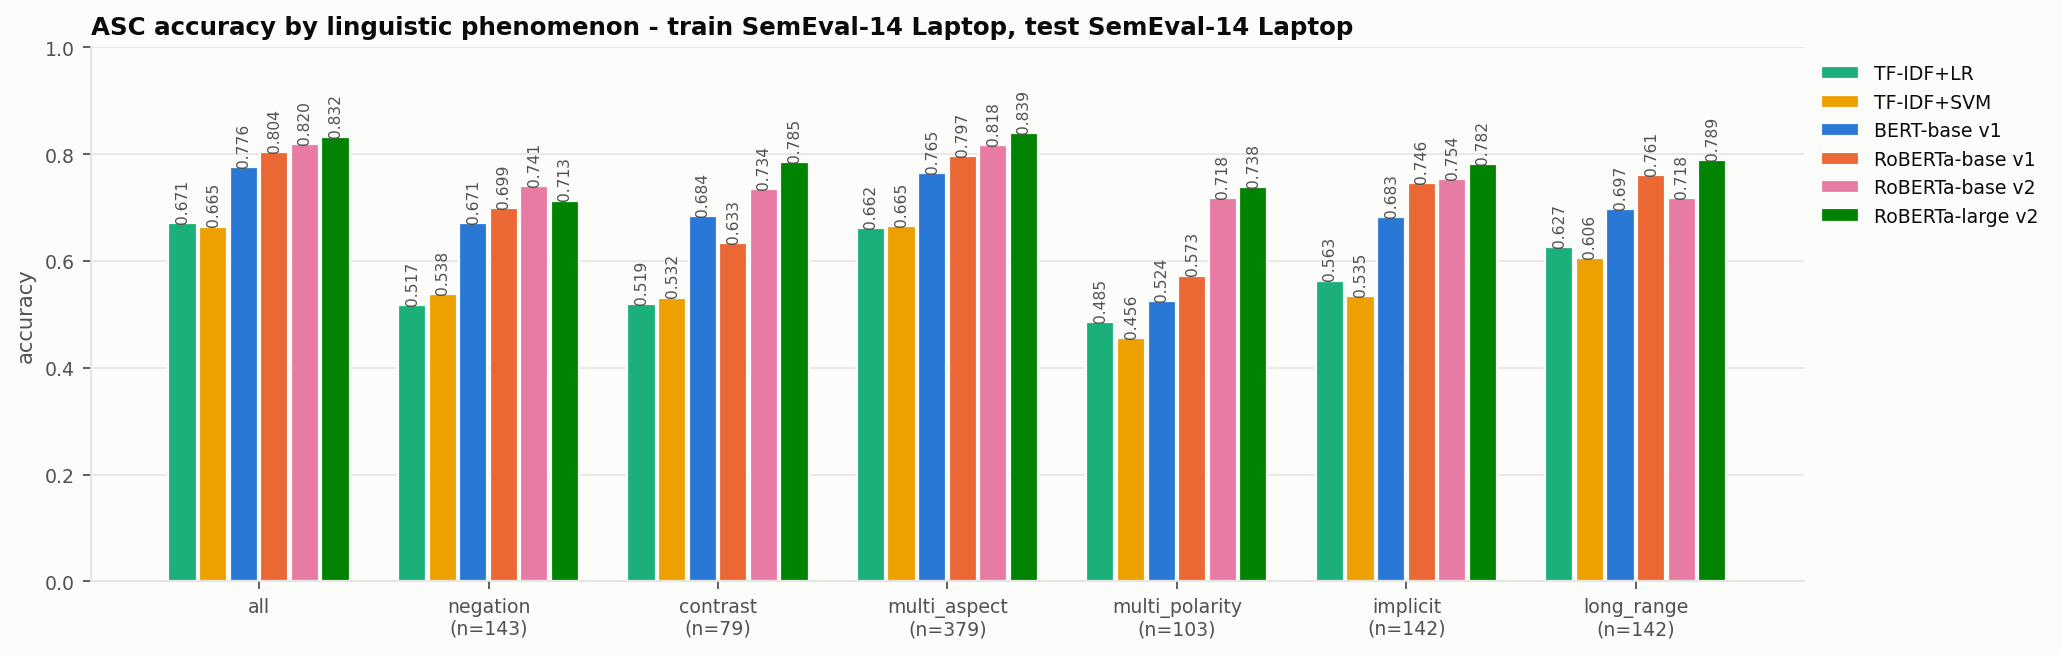
\includegraphics[width=0.49\textwidth]{figures/phenomena_semeval.png}
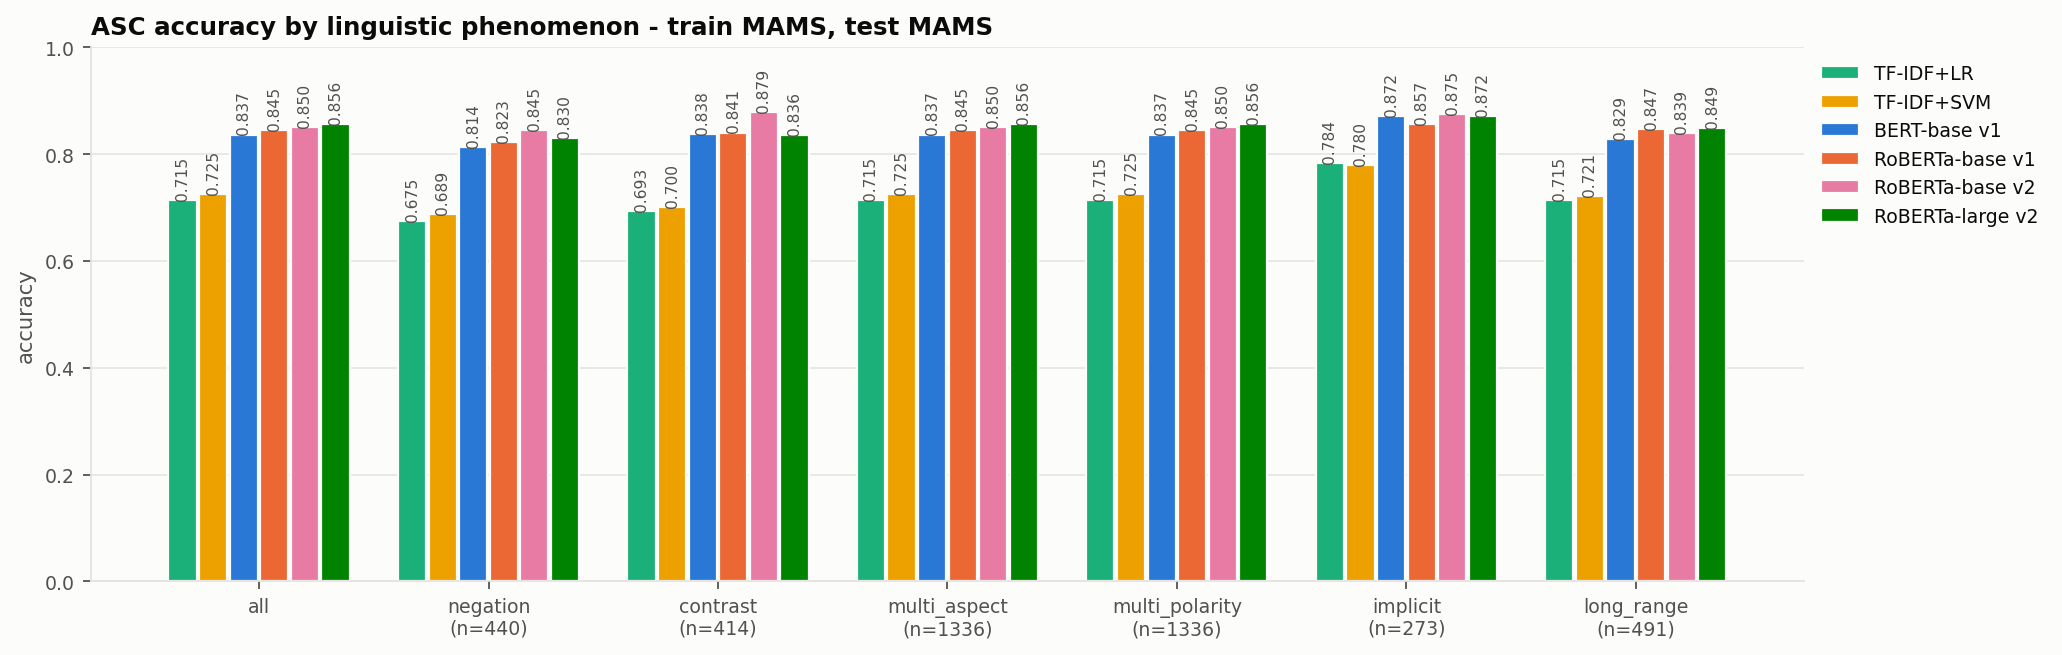
\includegraphics[width=0.49\textwidth]{figures/phenomena_mams.png}
\caption{Sentiment accuracy for each group of test examples, Laptops (left) and MAMS (right).}
\label{fig:phen}
\end{figure*}

\textbf{Implicit and long-range sentiment.} Aspects in sentences with no opinion words reach 78.2\% on Laptops, and aspects far away from their opinion word 78.9\%. Implicit sentiment is often stated as a fact, like ``it shuts down after an hour'', and realising that this is bad needs some knowledge of the world.

\textbf{Confusions.} Figure~\ref{fig:confusion} shows the confusion matrices of RoBERTa-large v2. On Laptops, 89\% of its 107 mistakes involve the neutral class, either as the true label or as the prediction, while mixing up positive and negative is much rarer. Table~\ref{tab:examples} lists some typical mistakes. The first two show what still goes wrong: in ``Did not enjoy the new Windows 8\ldots{}'' the model misses the negation, and in ``I can refute that OSX is FAST'' it misses that the writer is disagreeing with a claim.

\begin{figure}[t]
\centering
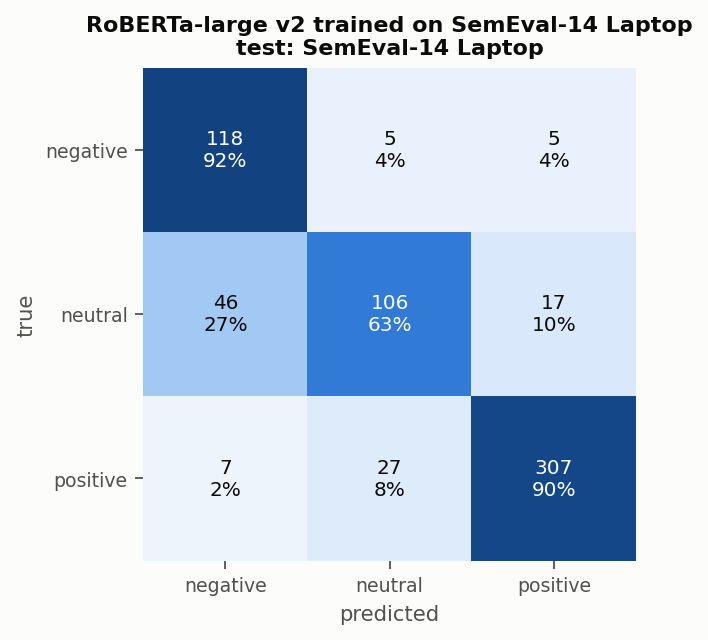
\includegraphics[width=0.49\columnwidth]{figures/confusion_large_semeval.png}
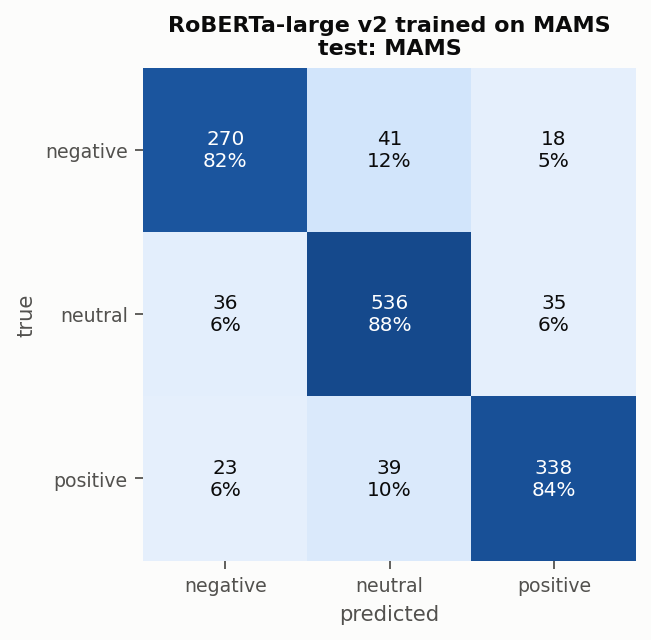
\includegraphics[width=0.49\columnwidth]{figures/confusion_large_mams.png}
\caption{Confusion matrices of RoBERTa-large v2 on Laptops (left) and MAMS (right).}
\label{fig:confusion}
\end{figure}

\begin{table*}[t]
\centering
\footnotesize
\begin{tabular}{p{0.52\textwidth}p{0.14\textwidth}p{0.10\textwidth}p{0.11\textwidth}p{0.21\textwidth}}
\toprule
Sentence & Aspect & Gold & Predicted & Tags \\
\midrule
Did not enjoy the new Windows 8 and touchscreen functions. & \textit{Windows 8} & negative & positive & negation, multi-aspect \\
However, I can refute that OSX is "FAST". & \textit{OSX} & negative & positive & contrast \\
From the speed to the multi touch gestures this operating system beats Windows easily. & \textit{Windows} & negative & positive & multi-aspect, multi-polarity, implicit \\
The baterry is very longer. & \textit{baterry} & positive & negative & implicit \\
\bottomrule
\end{tabular}
\caption{Some mistakes of RoBERTa-large v2 on the Laptops test set.}
\label{tab:examples}
\end{table*}

\section{Conclusion}
We built an ABSA pipeline for aspect extraction and aspect sentiment and used it to compare TF-IDF models with fine-tuned Transformers on SemEval-2014 Laptops and MAMS. Three things stood out. First, pre-trained encoders are clearly better than bag-of-words models on both steps, and our best models reach 79.9 macro-F1 on Laptops and 85.1 on MAMS. Second, how well a model transfers depends mostly on what it was trained on. Training on MAMS, where every sentence mixes sentiments, gives a model that also works on Laptops. Training on Laptops does not prepare a model for MAMS, and aspect extraction does not carry over between the two domains at all. Third, a second round of training based on what the first-round curves showed improved most in-domain results and the hard Laptops-to-MAMS setting, and a larger encoder added a little more on top. The biggest single gain came on Laptops sentences that mix positive and negative opinions, the group our first models handled worst. Negation is now the main weak spot.

If we continued this work, we would average our results over several seeds, continue pre-training the encoders on unlabelled reviews from both domains, train one model on both datasets together, and replace the two-step pipeline with a single model that finds aspects and their sentiment at the same time.

\section*{Limitations}
All results come from one random seed per setting, so differences of one or two points may not be meaningful. The phenomenon tags in the error analysis come from simple rules and a word list, not from manual annotation, and will be wrong for some sentences. Dropping the SemEval conflict class makes the task a little easier than the original four-class version. We set the v2 hyper-parameters by hand from the v1 curves rather than with a proper search. Finally, both datasets are in English and cover only two domains, so our conclusions about transfer may not hold for other languages or product types.

\section*{Use of AI Assistants}
We used an AI assistant to help write the experiment code and to help draft and edit this report. The project idea and the choice of datasets and methods come from our proposal, and every number in this report comes from running our code.

\begin{thebibliography}{99}
\expandafter\ifx\csname natexlab\endcsname\relax\def\natexlab#1{#1}\fi
\bibitem[{Devlin et~al.(2019)}]{devlin2019bert}
Jacob Devlin, Ming-Wei Chang, Kenton Lee, and Kristina Toutanova. 2019. BERT: Pre-training of deep bidirectional transformers for language understanding. In \textit{Proceedings of NAACL-HLT}, pages 4171--4186.

\bibitem[{Hu and Liu(2004)}]{hu2004mining}
Minqing Hu and Bing Liu. 2004. Mining and summarizing customer reviews. In \textit{Proceedings of the 10th ACM SIGKDD International Conference on Knowledge Discovery and Data Mining}, pages 168--177.

\bibitem[{Jiang et~al.(2019)}]{jiang2019mams}
Qingnan Jiang, Lei Chen, Ruifeng Xu, Xiang Ao, and Min Yang. 2019. A challenge dataset and effective models for aspect-based sentiment analysis. In \textit{Proceedings of EMNLP-IJCNLP}, pages 6280--6285.

\bibitem[{Liu(2012)}]{liu2012sentiment}
Bing Liu. 2012. \textit{Sentiment Analysis and Opinion Mining}. Morgan \& Claypool Publishers.

\bibitem[{Liu(2015)}]{liu2015sentiment}
Bing Liu. 2015. \textit{Sentiment Analysis: Mining Opinions, Sentiments, and Emotions}. Cambridge University Press.

\bibitem[{Liu et~al.(2019)}]{liu2019roberta}
Yinhan Liu, Myle Ott, Naman Goyal, Jingfei Du, Mandar Joshi, Danqi Chen, Omer Levy, Mike Lewis, Luke Zettlemoyer, and Veselin Stoyanov. 2019. RoBERTa: A robustly optimized BERT pretraining approach. \textit{arXiv preprint arXiv:1907.11692}.

\bibitem[{Medhat et~al.(2014)}]{medhat2014sentiment}
Walaa Medhat, Ahmed Hassan, and Hoda Korashy. 2014. Sentiment analysis algorithms and applications: A survey. \textit{Ain Shams Engineering Journal}, 5(4):1093--1113.

\bibitem[{Miyato et~al.(2017)}]{miyato2017adversarial}
Takeru Miyato, Andrew M. Dai, and Ian Goodfellow. 2017. Adversarial training methods for semi-supervised text classification. In \textit{International Conference on Learning Representations}.

\bibitem[{Pang and Lee(2008)}]{pang2008opinion}
Bo Pang and Lillian Lee. 2008. Opinion mining and sentiment analysis. \textit{Foundations and Trends in Information Retrieval}, 2(1--2):1--135.

\bibitem[{Pontiki et~al.(2014)}]{pontiki2014semeval}
Maria Pontiki, Dimitris Galanis, John Pavlopoulos, Harris Papageorgiou, Ion Androutsopoulos, and Suresh Manandhar. 2014. SemEval-2014 task 4: Aspect based sentiment analysis. In \textit{Proceedings of the 8th International Workshop on Semantic Evaluation}, pages 27--35.

\bibitem[{Pontiki et~al.(2016)}]{pontiki2016semeval}
Maria Pontiki, Dimitris Galanis, Haris Papageorgiou, et al. 2016. SemEval-2016 task 5: Aspect based sentiment analysis. In \textit{Proceedings of the 10th International Workshop on Semantic Evaluation}, pages 19--30.

\bibitem[{Reimers and Gurevych(2019)}]{reimers2019sentence}
Nils Reimers and Iryna Gurevych. 2019. Sentence-BERT: Sentence embeddings using Siamese BERT-networks. In \textit{Proceedings of EMNLP-IJCNLP}.

\bibitem[{Rietzler et~al.(2020)}]{rietzler2020adapt}
Alexander Rietzler, Sebastian Stabinger, Paul Opitz, and Stefan Engl. 2020. Adapt or get left behind: Domain adaptation through BERT language model finetuning for aspect-target sentiment classification. In \textit{Proceedings of the 12th Language Resources and Evaluation Conference}.

\bibitem[{Sun et~al.(2019)}]{sun2019utilizing}
Chi Sun, Luyao Huang, and Xipeng Qiu. 2019. Utilizing BERT for aspect-based sentiment analysis via constructing auxiliary sentence. In \textit{Proceedings of NAACL-HLT}.

\bibitem[{Szegedy et~al.(2016)}]{szegedy2016rethinking}
Christian Szegedy, Vincent Vanhoucke, Sergey Ioffe, Jon Shlens, and Zbigniew Wojna. 2016. Rethinking the inception architecture for computer vision. In \textit{Proceedings of CVPR}.

\bibitem[{Turney(2002)}]{turney2002thumbs}
Peter D. Turney. 2002. Thumbs up or thumbs down? Semantic orientation applied to unsupervised classification of reviews. In \textit{Proceedings of ACL}, pages 417--424.

\bibitem[{Vaswani et~al.(2017)}]{vaswani2017attention}
Ashish Vaswani, Noam Shazeer, Niki Parmar, Jakob Uszkoreit, Llion Jones, Aidan N. Gomez, {\L}ukasz Kaiser, and Illia Polosukhin. 2017. Attention is all you need. In \textit{Advances in Neural Information Processing Systems}.

\bibitem[{Zhou and Chen(2022)}]{zhou2022improved}
Wenxuan Zhou and Muhao Chen. 2022. An improved baseline for sentence-level relation extraction. In \textit{Proceedings of AACL-IJCNLP}.

\end{thebibliography}
\end{document}